\section{Goldstone's theorem}

\begin{figure}
    \centering
    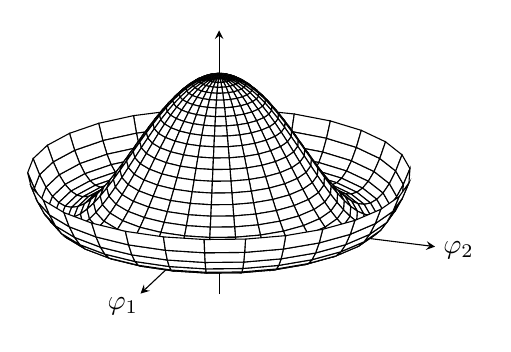
\begin{tikzpicture}
        \begin{axis}[
            axis lines=center,
            axis on top = false,
            view={110}{20},
            axis equal,
            % title={The Mexican hat potential},
            samples=30,
            domain=0:360,
            x label style={at={(0.296,0.1)}},
            y label style={at={(0.95,0.27)}},
            ymax = 1.5,
            xmax = 1.5,
            y domain=0:1.25,
            zmin=0,
            zmax=0.8,
            xlabel=$\varphi_1$,
            ylabel=$\varphi_2$,
            zlabel=$\Ve$,
            ticks=none,
        ]
        \addplot3 [
            surf, shader=flat, draw=black, fill=white, z buffer=sort
            ] ({sin(x)*y}, {cos(x)*y}, {(y^2-1)^2});
        \end{axis}
    \end{tikzpicture}
    \label{fig:Mexican hat}
    \caption{The Mexican hat potential.}
\end{figure}


The ground state of a theory is not necessarily invariant under the symmetry transformations of the theory.
This is exemplified by the linear sigma model,
\begin{equation}
    \Ell[\varphi] 
    = \frac{1}{2} \partial_\mu \varphi_i(x) \partial^\mu \varphi_i(x) - \Ve[\varphi],
    \quad \Ve[\varphi] = - \frac{1}{2} \mu^2 \varphi_i(x)\varphi_i(x)
    + \frac{1}{4} \lambda [\varphi_i(x) \varphi_i(x)]^2.
\end{equation}
This Lagrangian is invariant under the rotation of the $N$ fields,
\begin{equation}
    \varphi_i \longrightarrow \varphi_i' = O_{ij} \varphi_j,
    \quad O^{-1} = O^{T}.
\end{equation}
The set of all such rotation matrices is the Lie group $O(N)$. (SKRIVE APPENDIX OM LIE GRUPPER?)
If we assume the ground state $\varphi_{0}$ is translationally invariant, then it is give by minimizing the effective potential.
The first approximation of this is given by the classical potential, $\Ve$.
For $N=2$, this is the famous ``Mexican hat''-potential, as illustrated by \autoref{fig:Mexican hat}.
The ground state is therefore given by any of the values along the brim of the potential.
If we, without loss of generality, choose $\varphi = (0, v)$ as the ground state, then any symmetry transformation will change this state.
We say that the symmetry has been \emph{spontaneously broken}.
We can express this mathematically as
\begin{equation}
    \ex{ g_i[\varphi] }_0 \neq 0.
\end{equation}

If we take the constraint \cref{effective equation of motion}, differentiate with respect to $\varphi_j$ and evaluate in the vacuum, we get
\begin{equation}
    \int \dd^4 x \, \fdiff{\Gamma[\varphi_0]}{\varphi_j(x) \varphi_i(x)}
    t_{ik} \ex{\varphi_k}_0 = 0.
\end{equation}
